\documentclass[tikz,border=6pt]{standalone}
\usepackage[T1]{fontenc}
\usepackage{lmodern}
\usetikzlibrary{positioning,arrows.meta,calc}
\definecolor{tr}{HTML}{30638E}
\definecolor{te}{HTML}{D1495B}
\begin{document}
\sffamily\footnotesize
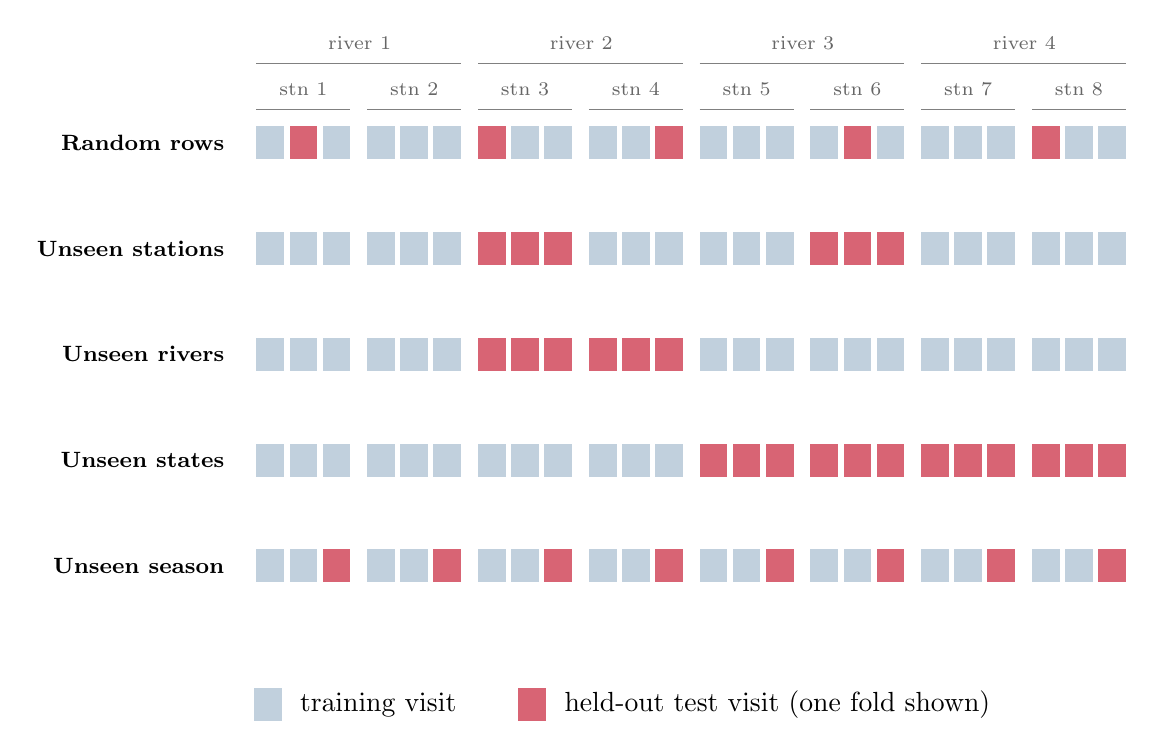
\begin{tikzpicture}[x=4.2mm,y=4.2mm]
% 5 schemes, each a grid of 24 "visits": columns grouped into stations, stations into rivers
\def\schemes{{"Random rows","Unseen stations","Unseen rivers","Unseen states","Unseen season"}}
\foreach \s [count=\k from 0] in {0,1,2,3,4}{
  \pgfmathsetmacro{\yy}{-\k*3.2}
  \pgfmathparse{\schemes[\k]}\let\name\pgfmathresult
  \node[anchor=east, font=\footnotesize\bfseries] at (-0.6,\yy+0.5) {\name};
  \foreach \i in {0,...,23}{
    % station = i div 3 (8 stations), river = i div 6 (4 rivers), state = i div 12 (2 states), season = i mod 3
    \pgfmathtruncatemacro{\st}{div(\i,3)}
    \pgfmathtruncatemacro{\rv}{div(\i,6)}
    \pgfmathtruncatemacro{\sa}{div(\i,12)}
    \pgfmathtruncatemacro{\se}{mod(\i,3)}
    \pgfmathtruncatemacro{\rnd}{mod(\i*7+3,5)}
    \ifcase\k
      \pgfmathtruncatemacro{\test}{\rnd==0 ? 1 : 0}
    \or
      \pgfmathtruncatemacro{\test}{(\st==2 || \st==5) ? 1 : 0}
    \or
      \pgfmathtruncatemacro{\test}{\rv==1 ? 1 : 0}
    \or
      \pgfmathtruncatemacro{\test}{\sa==1 ? 1 : 0}
    \or
      \pgfmathtruncatemacro{\test}{\se==2 ? 1 : 0}
    \fi
    \ifnum\test=1
      \fill[te!85] (\i+0.08+\st*0.35,\yy) rectangle ++(0.84,1);
    \else
      \fill[tr!30] (\i+0.08+\st*0.35,\yy) rectangle ++(0.84,1);
    \fi
  }
}
% grouping braces at top
\foreach \st in {0,...,7}{
  \draw[black!50] (\st*3+0.08+\st*0.35,1.5) -- ++(2.84,0);
  \node[font=\scriptsize, text=black!60] at (\st*3+1.5+\st*0.35,2.1) {stn \the\numexpr\st+1\relax};
}
\foreach \rv in {0,...,3}{
  \draw[black!50] (\rv*6+0.08+\rv*0.7,2.9) -- ++(6.19,0);
  \node[font=\scriptsize, text=black!60] at (\rv*6+3.2+\rv*0.7,3.5) {river \the\numexpr\rv+1\relax};
}
\fill[tr!30] (0,-17) rectangle ++(0.84,1); \node[anchor=west] at (1.1,-16.5) {training visit};
\fill[te!85] (8,-17) rectangle ++(0.84,1); \node[anchor=west] at (9.1,-16.5) {held-out test visit (one fold shown)};
\end{tikzpicture}
\end{document}
